\chapter{Implementation into ASLA}

In this chapter, it is attempted to implement the structure filter from the previous chapter into the Atomistic Structure Learning Algorithm (ASLA). 

\section{Hyperparameter search}
\begin{figure}
	\centering
	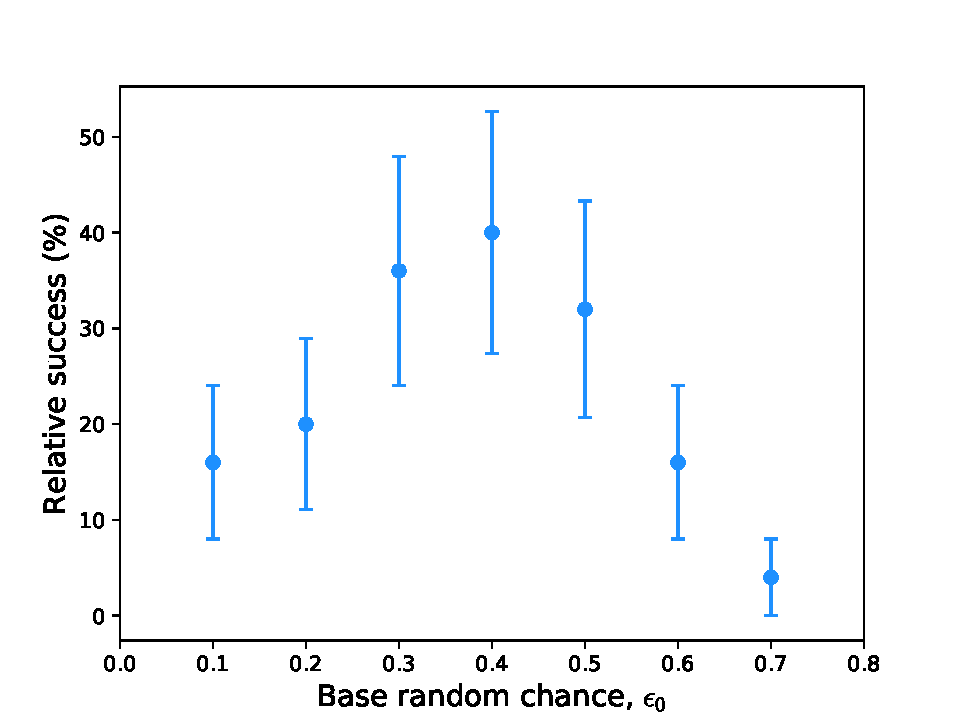
\includegraphics[width=0.8\columnwidth]{graphics/hypersearch_epsilon.pdf}
	\caption{The chance to make a completely random action during $\epsilon$-policy builds, $\epsilon_0$, was varied between $1/10$ through $7/10$. After initiating 25 agents with each value of $\epsilon_0$, the number of agents that found the global minimum solution were counted. The figure shows that the setting $\epsilon_0 = 4/10$ proved the most fruitful.}
	\label{fig:epsilon_variation}
\end{figure}

Before implementing the filter, it was firstly attempted to determine the best ratio of exploration/exploitation for the 'baseline' ASLA, which the filter will attempt to improve. Recall from chapter 2 that the parameter $\epsilon_0$, used during the $\epsilon$-policy builds, determines the chance for an action to randomly place an atom on the grid. To determine the optimal value of $\epsilon_0$, 25 instances of ASLA were initiated with a run time limit of either 5000 episoded or maximum time limit of $\SI{24}{\hour}$. After all instances had finished running, it was checked how many of the instances that had found the global minimum structure. The random chance was varied between $10\%$ up to $70\%$ and the results can be seen on figure \ref{fig:epsilon_variation}. From the figure it can be seen that $\epsilon_0 = 4/10$ is the most fruitful setting, which is then used for all future instances of ASLA.



\section{Method}
To implement the filter into ASLA, a new build-policy is made, which will be called the $\epsilon$-loop policy. Furthermore, ASLA will calculate and save the global feature vector of the latest 500 structures along with their DFT energies, so that each episode above $500$ will have an \bm{$\varepsilon$} to estimate future structure energies. Then, whenever the build-policy is $\epsilon$, the new $\epsilon$-loop policy will $80\%$ of the time be chosen as the build policy instead. During the $\epsilon$-loop policy, the agent will be asked to build 50 structures with the $\epsilon$ policy, but not complete the expensive DFT calculation for the structure. Each of the returned builds are saved and their energies are estimated using the current \bm{$\varepsilon$}. The structures are then sorted, and a final candidate is chosen among the 50\% of candidates with lowest estimated energies. The final structure is then treated as the only structure built by the agent that episode, and DFT energy calculation and training is done as usual.

\section{Results}
\begin{figure}
	\centering
	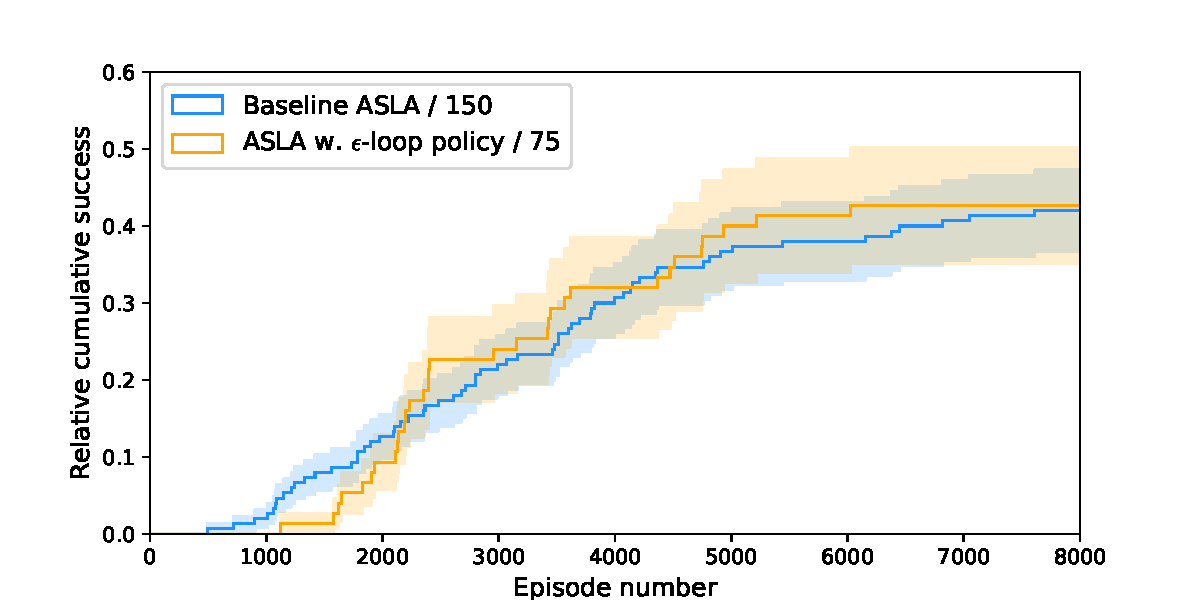
\includegraphics[width=\columnwidth]{graphics/S_curve.pdf}
	\captionsetup{width=1.3\columnwidth}
	\caption{Resulting S-curve comparing the cumulative success of each type of agent to the episode in which the solution is found. The agents have a limit of 10,000 episodes or \SI{24}{\hour}. As can be seen on the figure, the $\epsilon$-loop agents all find the global solution significantly slower than the baseline. However, the $\epsilon$-loop agents end up with the same fraction of agents finding the global solution as the baseline. Since the uncertainties of the 2 types of agents overlap after episode 2500, we cannot claim that the performance of one agent is significantly different from the others after that episode.}
	\label{fig:S-curve}
\end{figure}

After running both baseline ASLA agents and ASLA agents with the $\epsilon$-loop policy, the number of agents that found the global minimum solution were counted. The performance of both algorithms are compared and illustrated in figure \ref{fig:S-curve}. As can be seen on the figure, the performance of the $\epsilon$-loop agents are equal to if not slightly worse than their baseline counterparts. Due to the uncertainty of the performance results, the two algorithms cannot be said to be significantly different from each other, and so, it cannot be claimed that the $\epsilon$-loop implementation improves the performance of ASLA. Due to the $\epsilon$-loop agents being significantly slower in finding solutions, it seems that the implementation of energy estimation during the early episodes of building will hinder the structure search, while at later episodes it will simply match the performance of the baseline ASLA. 






